
    \documentclass{standalone}
    \usepackage{tikz}

    \begin{document}

    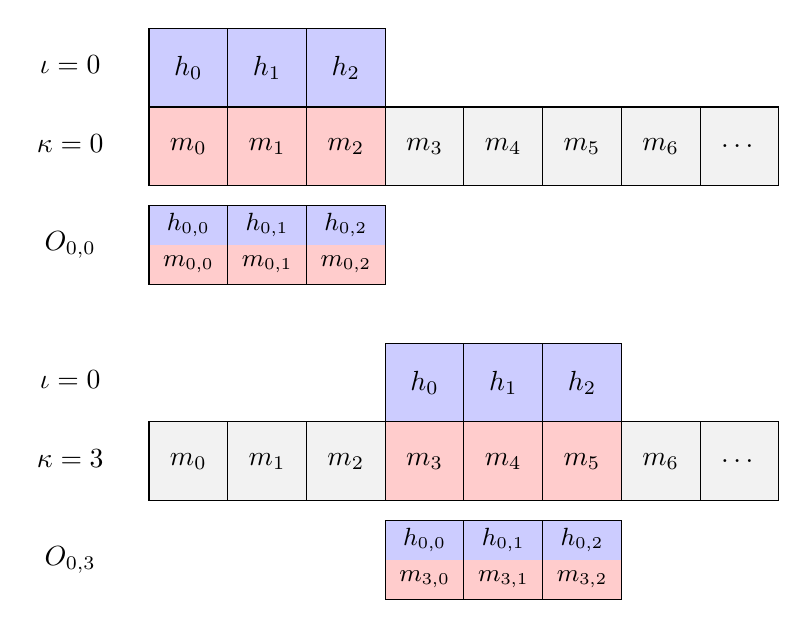
\begin{tikzpicture}

    
\node[anchor=mid] at (-1, 0.5) {$\kappa=3$} ;
\node[anchor=mid] at (-1, -0.75) {$O_{0,3}$} ;
\draw[fill=gray!10] (0, 0) rectangle ++(1, 1);
\node at (0.5, 0.5) {$m_{0}$};
\draw[fill=gray!10] (1, 0) rectangle ++(1, 1);
\node at (1.5, 0.5) {$m_{1}$};
\draw[fill=gray!10] (2, 0) rectangle ++(1, 1);
\node at (2.5, 0.5) {$m_{2}$};
\draw[fill=red!20] (3, 0) rectangle ++(1, 1);
\node at (3.5, 0.5) {$m_{3}$};
\node[minimum width=1cm,minimum height=0.5cm,inner ysep=0,font=\small,fill=blue!20] at (3.5, -0.5) {$h_{0,{0}}$};
\node[minimum width=1cm,minimum height=0.5cm,inner ysep=0,font=\small,fill=red!20] at (3.5, -1) {$m_{3,{0}}$};
\draw (3, -1.25) rectangle ++ (1, 1);
\draw[fill=red!20] (4, 0) rectangle ++(1, 1);
\node at (4.5, 0.5) {$m_{4}$};
\node[minimum width=1cm,minimum height=0.5cm,inner ysep=0,font=\small,fill=blue!20] at (4.5, -0.5) {$h_{0,{1}}$};
\node[minimum width=1cm,minimum height=0.5cm,inner ysep=0,font=\small,fill=red!20] at (4.5, -1) {$m_{3,{1}}$};
\draw (4, -1.25) rectangle ++ (1, 1);
\draw[fill=red!20] (5, 0) rectangle ++(1, 1);
\node at (5.5, 0.5) {$m_{5}$};
\node[minimum width=1cm,minimum height=0.5cm,inner ysep=0,font=\small,fill=blue!20] at (5.5, -0.5) {$h_{0,{2}}$};
\node[minimum width=1cm,minimum height=0.5cm,inner ysep=0,font=\small,fill=red!20] at (5.5, -1) {$m_{3,{2}}$};
\draw (5, -1.25) rectangle ++ (1, 1);
\draw[fill=gray!10] (6, 0) rectangle ++(1, 1);
\node at (6.5, 0.5) {$m_{6}$};
\draw[fill=gray!10] (7, 0) rectangle ++(1, 1);
\node at (7.5, 0.5) {\dots};
\node[anchor=mid] at (-1, 1.5) {$\iota=0$};
\draw[fill=blue!20] (3, 1) rectangle ++(1, 1);
\node at (3.5, 1.5) {$h_{0}$};
\draw[fill=blue!20] (4, 1) rectangle ++(1, 1);
\node at (4.5, 1.5) {$h_{1}$};
\draw[fill=blue!20] (5, 1) rectangle ++(1, 1);
\node at (5.5, 1.5) {$h_{2}$};
\node[anchor=mid] at (-1, 4.5) {$\kappa=0$} ;
\node[anchor=mid] at (-1, 3.25) {$O_{0,0}$} ;
\draw[fill=red!20] (0, 4) rectangle ++(1, 1);
\node at (0.5, 4.5) {$m_{0}$};
\node[minimum width=1cm,minimum height=0.5cm,inner ysep=0,font=\small,fill=blue!20] at (0.5, 3.5) {$h_{0,{0}}$};
\node[minimum width=1cm,minimum height=0.5cm,inner ysep=0,font=\small,fill=red!20] at (0.5, 3) {$m_{0,{0}}$};
\draw (0, 2.75) rectangle ++ (1, 1);
\draw[fill=red!20] (1, 4) rectangle ++(1, 1);
\node at (1.5, 4.5) {$m_{1}$};
\node[minimum width=1cm,minimum height=0.5cm,inner ysep=0,font=\small,fill=blue!20] at (1.5, 3.5) {$h_{0,{1}}$};
\node[minimum width=1cm,minimum height=0.5cm,inner ysep=0,font=\small,fill=red!20] at (1.5, 3) {$m_{0,{1}}$};
\draw (1, 2.75) rectangle ++ (1, 1);
\draw[fill=red!20] (2, 4) rectangle ++(1, 1);
\node at (2.5, 4.5) {$m_{2}$};
\node[minimum width=1cm,minimum height=0.5cm,inner ysep=0,font=\small,fill=blue!20] at (2.5, 3.5) {$h_{0,{2}}$};
\node[minimum width=1cm,minimum height=0.5cm,inner ysep=0,font=\small,fill=red!20] at (2.5, 3) {$m_{0,{2}}$};
\draw (2, 2.75) rectangle ++ (1, 1);
\draw[fill=gray!10] (3, 4) rectangle ++(1, 1);
\node at (3.5, 4.5) {$m_{3}$};
\draw[fill=gray!10] (4, 4) rectangle ++(1, 1);
\node at (4.5, 4.5) {$m_{4}$};
\draw[fill=gray!10] (5, 4) rectangle ++(1, 1);
\node at (5.5, 4.5) {$m_{5}$};
\draw[fill=gray!10] (6, 4) rectangle ++(1, 1);
\node at (6.5, 4.5) {$m_{6}$};
\draw[fill=gray!10] (7, 4) rectangle ++(1, 1);
\node at (7.5, 4.5) {\dots};
\node[anchor=mid] at (-1, 5.5) {$\iota=0$};
\draw[fill=blue!20] (0, 5) rectangle ++(1, 1);
\node at (0.5, 5.5) {$h_{0}$};
\draw[fill=blue!20] (1, 5) rectangle ++(1, 1);
\node at (1.5, 5.5) {$h_{1}$};
\draw[fill=blue!20] (2, 5) rectangle ++(1, 1);
\node at (2.5, 5.5) {$h_{2}$};


    \end{tikzpicture}

    \end{document}

    
